% Local display/float spacing accommodates the boundary schematic; body type and leading are unchanged.
\begingroup
\setlength{\parskip}{0pt plus 1pt}
\setlength{\abovedisplayskip}{4pt plus 2pt minus 1pt}
\setlength{\belowdisplayskip}{4pt plus 2pt minus 1pt}
\setlength{\abovedisplayshortskip}{4pt plus 1pt minus 1pt}
\setlength{\belowdisplayshortskip}{4pt plus 1pt minus 1pt}
\setlength{\textfloatsep}{8pt plus 2pt minus 2pt}
\setlength{\intextsep}{8pt plus 2pt minus 2pt}
\setlength{\floatsep}{8pt plus 2pt minus 2pt}
\captionsetup{skip=5pt}
\renewcommand{\arraystretch}{1.0}
\section{问题一：预热阶段的径向分布}
\label{sec:q1}

问题一以第\ref{sec:common-model}节的统一模型为基础，在固定几何、常热物性条件下，
采用附录2物性预测前$1800\unit{s}$的径向温度与含水率分布。
水分扩散系数仍随含水率变化，两场分别求解；从参数代入到规定结果输出的过程如图\ref{fig:q1-workflow}所示。

\begingroup
\setlength{\intextsep}{10pt}
\begin{figure}[H]
\centering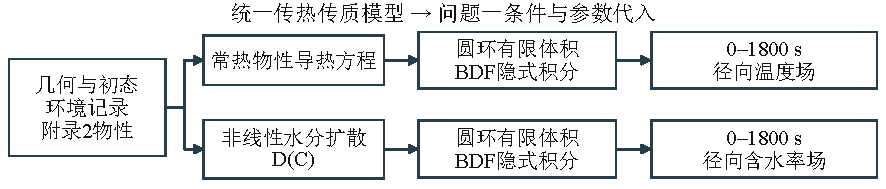
\includegraphics[width=\linewidth]{figures/legibility_schematics/q1_workflow.pdf}
\caption{问题一由统一模型到径向预热模型的求解流程}
\label{fig:q1-workflow}
\end{figure}
\endgroup

\subsection{常热物性方程与初边值条件}
题设圆柱药材长$25\unit{cm}$、半径$2\unit{cm}$。
本问取固定骨架$v_s=0$，式\eqref{eq:heat}、\eqref{eq:moisture}中的材料导数退化为时间偏导数。
初始干密度空间均匀且干物质守恒，故固定骨架下干密度保持均匀，可从水分方程约去。

依假设\ref{ass:midsection}取中截面径向近似并忽略端面影响，以$r,t$描述两场，
计算区间为$0\leq r\leq R$。轴心取零径向梯度，表面通过线性换热、传质关系与环境相联系。
几何与边界条件见图\ref{fig:q1-boundary}。

\begin{figure}[htbp]
\centering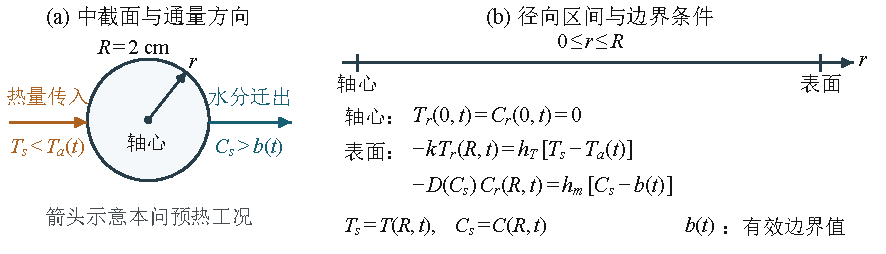
\includegraphics[width=\linewidth]{figures/legibility_schematics/q1_boundary.pdf}
\caption{问题一中截面径向模型与边界条件示意图}
\label{fig:q1-boundary}
\end{figure}

代入附录2的常热物性参数与扩散系数关系，得到径向导热方程与非线性水分扩散方程：
\begin{equation}
\begin{aligned}
T_t&=\alpha\frac{1}{r}\frac{\partial}{\partial r}(rT_r),
&\alpha&=\frac{0.36}{820\times2600},\\
C_t&=\frac{1}{r}\frac{\partial}{\partial r}\bigl(rD(C)C_r\bigr),
&D(C)&=7\times10^{-9}e^{-0.89/C}.
\end{aligned}
\label{eq:q1-pde}
\end{equation}
式\eqref{eq:q1-pde}定义在$0<r<R=0.02\unit{m}$，初态为
$T(r,0)=28\celsius$、$C(r,0)=2.55\unit{kg/kg}$。式\eqref{eq:boundary}
在轴线对称性和圆柱表面外法向下具体写为
\begin{equation}
\begin{aligned}
T_r(0,t)&=C_r(0,t)=0,\\
-0.36T_r(R,t)&=25[T(R,t)-T_a(t)],\\
-D(C_s)C_r(R,t)&=8\times10^{-7}[C_s-b(t)],\qquad C_s=C(R,t).
\end{aligned}
\label{eq:q1-bc}
\end{equation}
其中$T_a,b$由环境记录线性插值得到。本问的$D$不依赖温度，热方程也
不依赖含水率，因此两个场分别求解；水分场仍是非线性的，因为其散度
展开后为$D(C)(C_{rr}+C_r/r)+D'(C)C_r^2$，不能按常扩散率处理。
均匀初态与式\eqref{eq:q1-bc}在初始表面角点不相容，故保留题给初值，
允许$t>0$形成早期边界层，不人为调整初始表面含水率。

\subsection{圆环守恒离散与隐式求解}
为同时说明两个场的计算，记$u=T$时$a(u)=\alpha$、
$\beta=25/(820\times2600)$、$u_a=T_a$；$u=C$时$a(u)=D(u)$、
$\beta=8\times10^{-7}$、$u_a=b$。取节点$r_i=i\Delta r$，
$i=0,\ldots,N$、$\Delta r=R/N$，内部控制体面位于相邻节点中点，
两端面分别为$r_{-1/2}=0$、$r_{N+1/2}=R$。令外向加权通量
$G=-ra(u)u_r$，将式\eqref{eq:q1-pde}乘$r$并在圆环控制体内积分，得
\begin{equation}
\frac{\dd}{\dd t}\int_{r_{i-1/2}}^{r_{i+1/2}}ru\,\dd r
=G(r_{i-1/2},t)-G(r_{i+1/2},t).
\label{eq:q1-ring}
\end{equation}
真实体积中的公因子$2\pi L$已约去。以节点值近似式\eqref{eq:q1-ring}
的储存量，权重为$w_i=(r_{i+1/2}^2-r_{i-1/2}^2)/2$，因此轴心和
表面节点均保留各自控制体容量。把相邻两半格的扩散阻力串联相加，
即$\Delta r/\widehat a=(\Delta r/2)/a(u_i)+(\Delta r/2)/a(u_{i+1})$，
内部面得到调和平均及通量：
\begin{equation}
\widehat a_{i+1/2}=\frac{2a(u_i)a(u_{i+1})}{a(u_i)+a(u_{i+1})},\qquad
G_{i+1/2}=r_{i+1/2}\widehat a_{i+1/2}\frac{u_i-u_{i+1}}{\Delta r}.
\label{eq:q1-flux}
\end{equation}
同一式\eqref{eq:q1-flux}同时用于相邻两格，结合式\eqref{eq:q1-bc}
即得到实际积分的常微分方程组
\begin{equation}
\begin{aligned}
w_i\dot u_i&=G_{i-1/2}-G_{i+1/2},\qquad i=0,\ldots,N,\\
G_{-1/2}&=0,\qquad G_{N+1/2}=R\beta(u_N-u_a).
\end{aligned}
\label{eq:q1-ode}
\end{equation}
轴心内面通量自然为零，式\eqref{eq:q1-ode}无须计算奇异的$1/r$。
逐格求和后内部面通量抵消，由$\sum_iw_i=R^2/2$可得
\begin{equation}
\frac{\dd}{\dd t}\left(\frac{2}{R^2}\sum_{i=0}^Nw_i u_i\right)
=-\frac{2\beta}{R}(u_N-u_a).
\label{eq:q1-balance}
\end{equation}
式\eqref{eq:q1-balance}把圆柱加权平均的变化与表面交换直接对应，
也是数值程序累计边界通量、检查离散总量一致性的依据。

将式\eqref{eq:q1-ode}写为$\dot{\boldsymbol u}=\boldsymbol F(t,\boldsymbol u)$，
使用自适应隐式BDF方法\cite{scipy}。每步的新状态由隐式残量及Newton修正确定：
\begin{equation}
\begin{aligned}
\boldsymbol{\mathcal R}(\boldsymbol u^{n+1})
&=\gamma_n\boldsymbol u^{n+1}-\boldsymbol q_n
-\Delta t_n\boldsymbol F(t_{n+1},\boldsymbol u^{n+1})=\boldsymbol0,\\
\left[\gamma_n I-\Delta t_n J_F\right]\delta\boldsymbol u
&=-\boldsymbol{\mathcal R}.
\end{aligned}
\label{eq:q1-bdf}
\end{equation}
这里$\gamma_n,\boldsymbol q_n$由积分阶数、步长和已知历史状态确定；
实际采用SciPy的变阶BDF实现及其精度修正，式\eqref{eq:q1-bdf}表示共同的
隐式求解结构。解析稀疏Jacobian $J_F=\partial\boldsymbol F/\partial\boldsymbol u$
保留$D'(C)=0.89D(C)/C^2$及调和平均的导数，
在非线性迭代中更新扩散率。积分在每个环境输入折点重启并传递末态。
正式径向区间数为10240，相对容差$2\times10^{-12}$，最大步长$3\unit{s}$；
$1\unit{s}$是输出间隔，不是积分固定步长。

\subsection{规定结果与预热规律}
表\ref{tab:q1-temperature}和表\ref{tab:q1-moisture}给出规定的七个时刻、
五个径向位置。\texttt{result1.xlsx}从第1秒至第1800秒，每隔
$0.1\unit{cm}$输出21个位置的温度和干基含水率，共75600个数值；
计算不提前舍入，输出统一显示四位小数。

\begin{table}[htbp]
\centering\small
\caption{30分钟内药材中截面温度（$^\circ$C）}
\label{tab:q1-temperature}
\input{tables/q1_temperature.tex}
\end{table}

\begin{table}[htbp]
\centering\small
\caption{30分钟内药材中截面干基含水率（kg/kg）}
\label{tab:q1-moisture}
\input{tables/q1_moisture.tex}
\end{table}

$1800\unit{s}$时轴心、表面温度分别为33.5753\celsius{}和
36.7856\celsius，均低于该时刻环境温度41.5130\celsius。表面先响应，
轴心因传导而滞后。由未舍入值计算，径向温差为$3.2102\unit{K}$。
同期表面含水率降至$1.5102\unit{kg/kg}$，轴心实际含水率约为
$2.5499924\unit{kg/kg}$，四位显示仍为2.5500；因此不能把表中轴心数字
未变解释为水分数学上严格不变。

\begin{figure}[htbp]
\centering
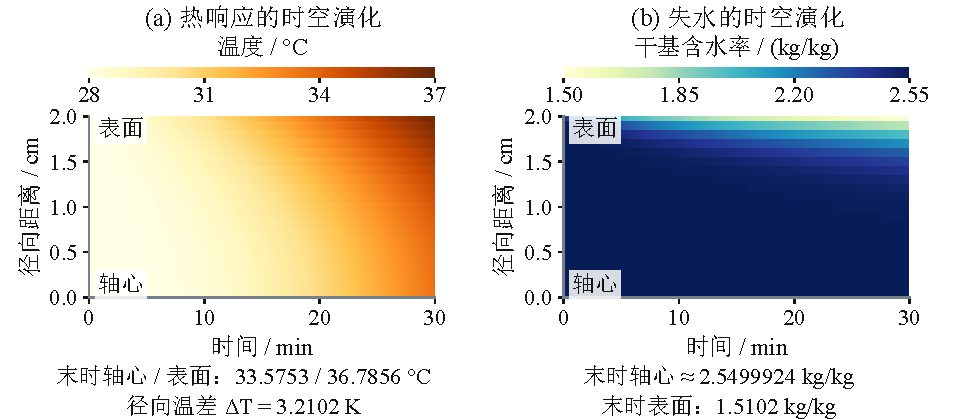
\includegraphics[width=0.94\textwidth]{figures/q1_legibility/q1_profiles.pdf}
\caption{第一问的时间--径向温湿场。横轴为时间，纵轴为径向距离；左、右色标分别表示温度与干基含水率，均由已保存采样值着色。}
\label{fig:q1-profiles}
\end{figure}

\Needspace{3\baselineskip}
沿图\ref{fig:q1-profiles}横向可跟踪同一径向位置的变化，沿纵向可比较同一时刻的内部与表面。色阶显示，升温已遍及所考察的径向位置，而水分变化
主要集中在表层。末时$r=1.5\unit{cm}$处的含水率为2.3755，较初值
下降约6.84\%，$r=1.0\unit{cm}$处仍为2.5383。这里不存在严格截断的
扩散前沿；描述受影响层厚度时需要先规定含水率变化阈值。

\Needspace{3\baselineskip}
以共同尺度$R$比较扩散时间：初始热扩散率
$\alpha=k/(\rho c_p)=1.6886\times10^{-7}\unit{m^2/s}$，
$D(C_0)=4.9377\times10^{-9}\unit{m^2/s}$，故
$R^2/\alpha=2368.89\unit{s}$、$R^2/D(C_0)=81010.11\unit{s}$，
两者相差34.20倍。这解释了预热阶段热响应快于水分响应；因失水使$D$
继续减小，初始扩散时间不是最终烘干时长。
圆柱平均须按$r\,\mathrm dr$加权，得到末时中截面平均温度
35.1679\celsius、平均含水率$2.2936\unit{kg/kg}$；它们不替代最湿点，
也不能直接当作包含端部效应的整根平均量。

\subsection{数值验证与适用范围}
针对前述温湿分布，先以独立参考检验数值一致性。
温度以贝塞尔特征函数展开作参考；
水分经$x=(r/R)^2$变换，以Chebyshev配点与非线性表面条件消元构造独立空间参考解。
正式解与参考解在全部规定输出点上的最大温度差为
$7.29\times10^{-9}\unit{K}$，含水率差为
$1.52\times10^{-6}\unit{kg/kg}$；全部75600个正式输出四位一致。

再检查时间积分精度的影响。固定正式网格收紧时间控制后，温湿差分别约
$5.03\times10^{-10}\unit{K}$和$8.15\times10^{-11}\unit{kg/kg}$。
接近舍入分界的数值必须逐项核对，不能仅凭最大误差小于半个末位单位
推断整张表四位一致。

为进一步检验忽略端面影响后的中截面径向近似，采用同物理条件下的$80\times128$有限圆柱二维模型进行配对比较。
在前$1800\unit{s}$已检查采样点上，中截面的最大温湿差分别约为
$5.65\times10^{-8}\unit{K}$与$4.09\times10^{-9}\unit{kg/kg}$，
支持本问中截面径向近似；端面局部差仍可较大，不能据此推广到整个圆柱。

独立核对与中截面配对为前述温湿分布提供了所选有效方程下的数值依据，
不消除等效湿度边界、参考密度
及无显式潜热假设引入的物理不确定性。
本问预热段的相变能量缺口量级显著，相关诊断与解释范围见第\ref{sec:limitations}节。
\FloatBarrier
\endgroup
